Web-Browser haben sich seit der Veröffentlichung von Mosaic, einer der ersten populären Browser, im Jahr 1993 stark weiterentwickelt \cite{EvolutionOfTheWebBrowser}. Das Abrufen und Anzeigen von statischen HTML-Dokumenten wurde mithilfe von JavaScript um interaktive und später um dynamische Inhalte erweitert. Heutzutage können Entwickler komplexe Webanwendungen realisieren \cite{SinglePageApplication}, welche zudem browserunabhängig entwickelt werden können. Durch diese Entwicklung und die vielseitigen Anwendungsfälle, besitzt die Umgebung \enquote{Browser} besondere Eigenschaften, welche nachfolgend beschrieben werden.

\subsection{Browserprodukte}
\label{sec:browserprodukte}

%\begin{wrapfigure}[19]{r}{0.45\textwidth}
%\centering
%\tikzsetnextfilename{cross-browser_metastudie.png}
%\begin{tikzpicture}
%	\begin{axis}[
%		ybar,
%        ymin=0,
%        ymax=300,
%        ytick distance={50},
%		area style,
%		legend style={at={(0.5,-0.10)},anchor=north},
%		nodes near coords,
%		symbolic x coords = {2015, 2016, 2017, 2018, 2019, 2020},
%	]
%		\addplot+[blue,fill opacity=0.2,text opacity=1,ybar,no marks]
%			plot coordinates {
%			(2015,272)
%			(2016,228)
%			(2017,208)
%			(2018,204)
%			(2019,172)
%			(2020,167)
%			};
%		\legend{\strut Suchtreffer bei Google Scholar}
%	\end{axis}
%\end{tikzpicture}
%\caption{Studien zur Browserkompatibilität, eigene Darstellung (vgl. \ref{sec:studien-zur-browser-kompatibilitaet})}
%\label{fig:studien-zur-browser-kompatibilitaet}
%\end{wrapfigure}

\begin{wrapfigure}[19]{r}{0.45\textwidth}
\centering
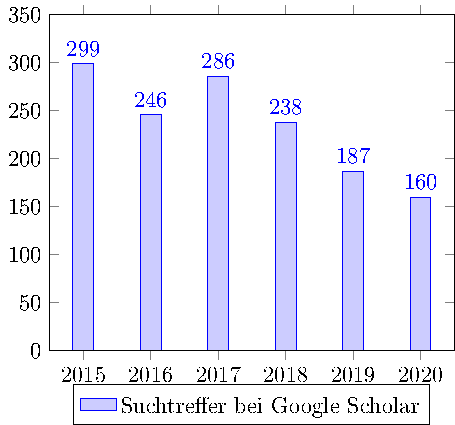
\includegraphics[width=\linewidth]{img/02_theorie/cross-browser_metastudie.png.pdf}
\caption{Studien zur Browserkompatibilität, eigene Darstellung (vgl. \autoref{sec:studien-zur-browser-kompatibilitaet})}
\label{fig:studien-zur-browser-kompatibilitaet}
\end{wrapfigure}

Die Vielfalt an Browsern bereitet Webentwicklern immer wieder eine Herausforderung, nämlich ob ein von ihnen bereitgestelltes Produkt für die Nutzer einwandfrei funktioniert, unabhängig der Browserpräferenz des Nutzers. Die Häufigkeit solcher Probleme, auch Cross-Browser-Incompatibilities (XBI) \cite{XBIs} genannt, hat jedoch abgenommen. Dies ist unter anderem durch den Trend von offenen Web-Standards, wie die des W3C \cite{W3CStandards}, erklärbar.

\nomenclature[Fachbegriff]{XBI}{Cross-Browser-Incompatibilities}

Generell lässt sich feststellen, dass auch in der Literatur die Veröffentlichungen in Bezug auf (In-)Kompatibilität von Browsern abnehmen, wie in \autoref{fig:studien-zur-browser-kompatibilitaet} zu betrachten. Dies spricht dafür, dass das Problem von XBIs weniger präsent ist als zuvor. Somit wird die besondere Hürde, die XBIs darstellen, nicht als relevante in dieser Arbeit angesehen.

Im Jahr 2020 gab es weitere Entwicklungen, die die Kompatibilität zwischen Browsern erhöhte. Microsoft ist beim Folgeprodukt zum Internet Explorer, dem Microsoft Edge Browser, von einer proprietären Browser-Engine zu Chromium gewechselt \cite{MicrosoftEdgeChromium} und verwendet denselben Kern wie Chrome und Opera. Zum 30.11.2020 stellte Microsoft zudem den Support für den Internet Explorer 11 ein \cite{MicrosoftInternetExplorerDeprecation}. Im Februar 2021 meldete StatCounter \cite{StatCounterBrowserMarketshare} eine Marktverteilung bei Desktop-Browsern von 66,47\% Chrome, 10,27\% Safari, 8,17\% Firefox, 8,01\% Edge, 2,68\% Opera und 1,89\% Internet Explorer.
